
\subsection{Implementation}
\begin{frame}[<+->]
\frametitle{Implementation}
\begin{itemize}
    \item A data type for functions real analytic on $[0,1]$ was implemented in \irram .
    \item Constructor from a single power series.
    \item Analytic continuation used if more series are needed to cover the interval. 
    \item The running time and memory usage was empirically analyzed.
    \item Running time increases quickly with number of analytic continuations. 
\end{itemize}
\end{frame}
\begin{frame}
  \frametitle{Evaluation\dots}
  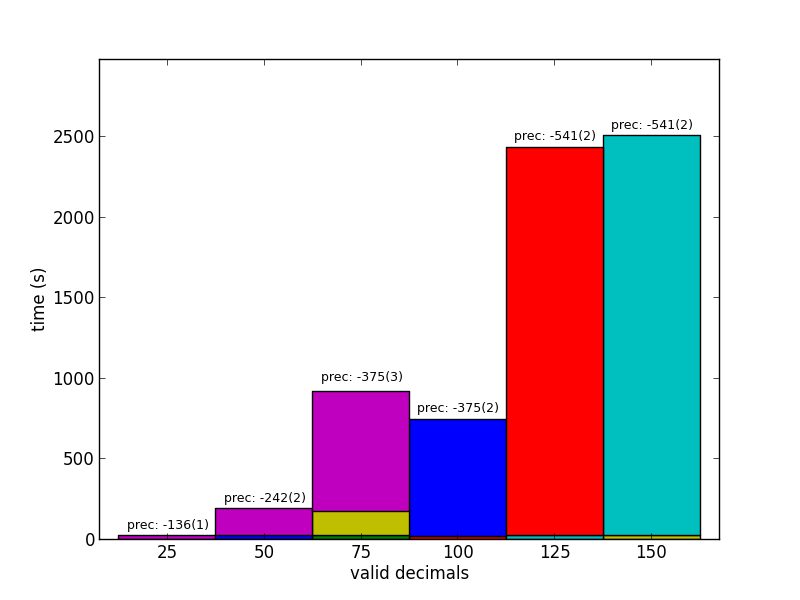
\includegraphics[width=0.9\textwidth]{sin_for_series_4_dep_on_n}
\end{frame}
\begin{frame}
  \frametitle{Evaluation\dots}
  \begin{minipage}{0.48\textwidth}
  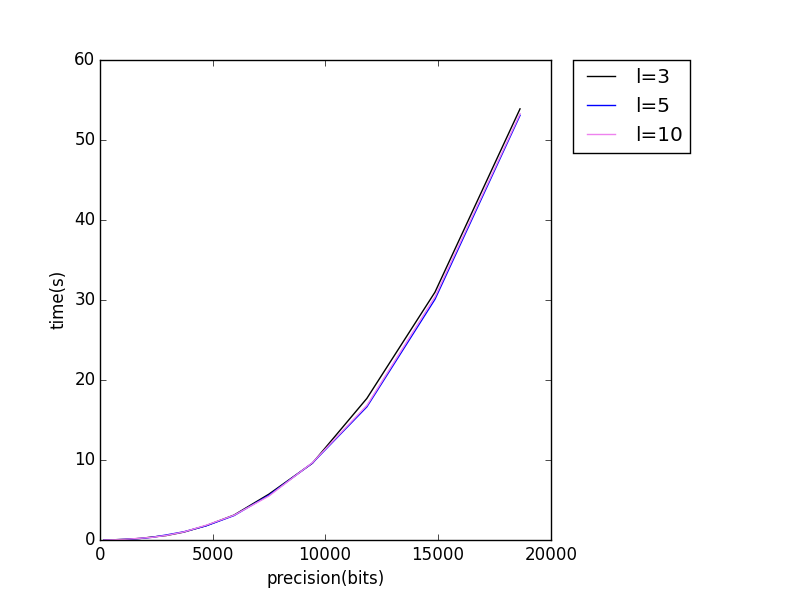
\includegraphics[width=1.2\textwidth]{time_0}
  \end{minipage}
  \begin{minipage}{0.48\textwidth}
  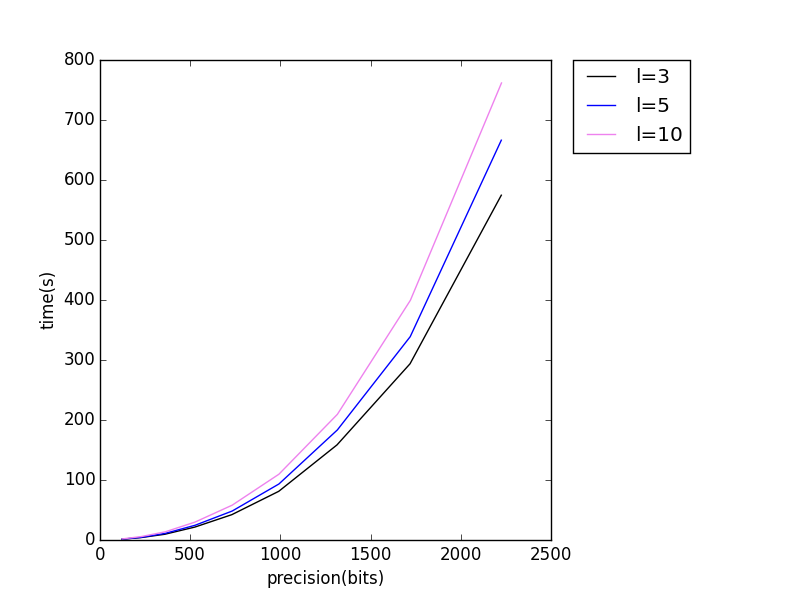
\includegraphics[width=1.2\textwidth]{time_1}
  \end{minipage}
\end{frame}
\begin{frame}
  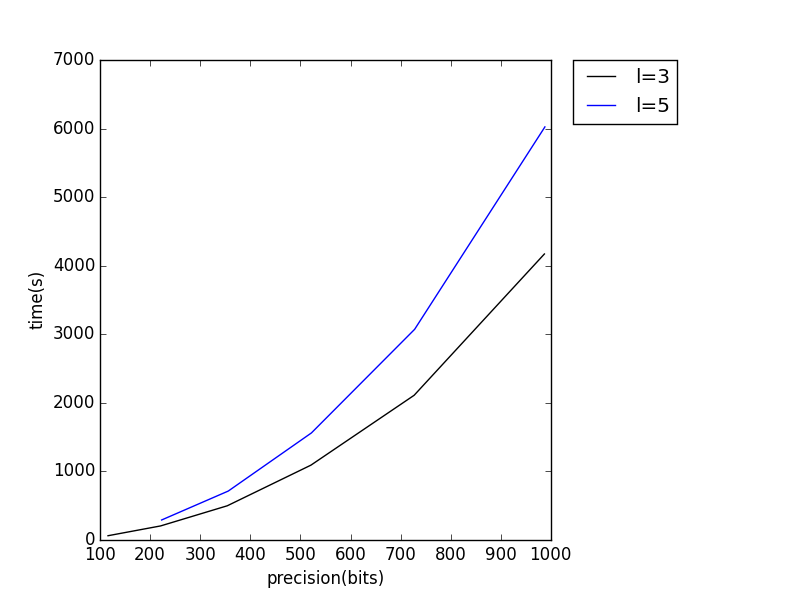
\includegraphics[width=0.8\textwidth]{time_2}
\end{frame}
\begin{frame}[t]{Riemann Mapping Theorem}
  \begin{theorem}[Riemann]
    Let $U \subsetneq \C$ be non empty, simply connected and open.\\
    Then there exists a biholomorphic mapping from $U$ on to the open unit disc.
%\begin{tikzpicture}[scale=0.9]
%    \path [use as bounding box,red] (-100pt,-10pt) rectangle (30pt,40pt);
%    \draw (-3,0.5) rectangle (2,-0.5);
%    \draw [thick,->] (2.2,0) -- (3.8,0);
%    \draw (5,0) ellipse (1cm and 1cm);
%\end{tikzpicture}
  \end{theorem}
\vfill
 How complex is it to compute this mapping?\\
  \pause
  In the general case $\#P$ hard (Binder, Braverman, Yampolsky).\\
  \pause
  Riemann mappings of domains with polynomial time computable analytic boundaries are polynomial time computable (Rettinger).
\end{frame}
\begin{frame}[<+->]{Summary}
 When developing Exact Real Arithmetic algorithms the following is important
 \begin{itemize}
     \item Careful mathematical analysis of the errors that arise by finite approximations has to be performed.
     \item Theorems from real and complex analysis have to be combined with methods from theoretical computer science to get efficient algorithms.
     \item Finding the right restriction of the type of functions considered, so that efficient algorithms are possible but the class still contains most functions relevant in practice.
     \item It is sometimes necessary to enrich the input by natural parameters of the function to gain better computability or complexity results.
 \end{itemize}
\end{frame}
